This is exactly what the Floyd Warshall algorithm does. It's a dynamic programming algorithm using three nested loops from 1 to $n$. Here's how it works.\\

The idea is to check for each pair of vertices ($v_i$ and $v_j$) the cost of travelling from one to another directly (without passing through another vertex). If there is no edge linking two vertices we set the cost to infinity. We can store those values in an array such that $path\_cost[i][j]$ equals this cost. To do so we can implement it using two nested loop one iterating $i$ from 1 to $n$ and the second for $j$ from 1 to $n$.\\
Now we want to calculate the cost from each pair of vertices passing through $v_1$. We then update $path\_cost[i][j]$ with the minimum between $path\_cost[i][j]$ and $path\_cost[i][1]+path\_cost[1][j]$. We do that $n$ times for each vertex. So we need to nest the two first loops in a new loop. We have then three nested loops, all from 1 to $n$ (we can either initialize the array $path\_cost$ before in a two nested loops or we can have the first loop starting from 0 to initialize the array). Thus the complexity is O($(n+1)\cdot n\cdot n$) $\leq$ O($n^3$).\\
\begin{figure}[ht]
  \centering
  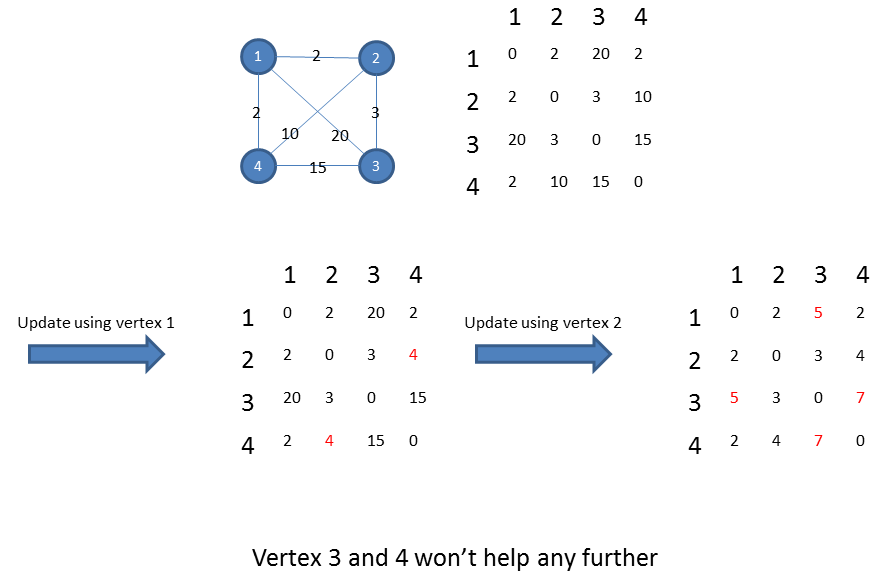
\includegraphics[width=1\textwidth]{q1}
  \caption{Execution of Floyd-Warshall}
  \label{fig:q2}
\end{figure}
\clearpage